\documentclass{article}
\usepackage{graphicx} % Required for inserting images
\usepackage{amsmath}
\usepackage{pgfplots}
\usepackage{tikz}
\usetikzlibrary{angles,quotes}
\usepackage{ amssymb }


\title{Remainder topics}
\author{Intro to Robotics}
\date{}

\begin{document}

\maketitle

\section{Inverse Manipulator Kinematics}
Kinematics is the science of motion that treats the subject without regard to the
forces that cause it. Within the science of kinematics, one studies the position, the
velocity, the acceleration, and all higher order derivatives of the position variables
(with respect to time or any other variable(s)). Hence, the study of the kinematics of
manipulators refers to all the geometrical and time-based properties of the motion.
\\\\
 Given the desired position and orientation of the tool relative to the
station, how do we compute the set of joint angles which will achieve this desired
result? \\\\
Solving the problem of finding the required joint angles to place the tool
frame, \{T\}, relative to the station frame, \{S\}, is split into two parts. First, frame
transformations are performed to find the wrist frame, \{W\}, relative to the base
frame, \{B\}, and then the inverse kinematics are used to solve for the joint angles.


\section{Jacobian Matrix and Singularities}
Definition of Jacobian - multidimensional matrix of derivatives(J$\rightarrow$ velocity differentiate from positions), Jacobians can relate the joint velocities to cartesian velocites in a robot manipulator.  \\\\
Cartesian: v=$\begin{bmatrix}
   \dot{ P_x} \\
    \dot{P_y} \\
    \dot{P_z}
\end{bmatrix}$ = Joint:$\begin{bmatrix}
                          {}^0v\\
                          {}^0w
\end{bmatrix} = J * \begin{bmatrix}
\dot{\theta_1} \\
\dot{\theta_2}
\end{bmatrix}$\\
${}^0v$ is linear\\
${}^0w$ is angular\\\\
You always need the jacobian in the base frame ${}^0J$, when you dont have it; you can solve for it. Use formula:\\
${}^0J={}^0_xR * {}^xJ$\\\\
Singularities- is a point where the robot loses one or more degrees of freedom. Here, it is impossible to move the end effector (tool) in a particular direction, regardless of the joint rates. two types: \\
\begin{itemize}
    \item Workspace-bound singularities- fully stretched out , or tool folded back on itself. Tool is at boundary of workspace.
    \item Workspace interior singularities - 2 or more joint axes line up with each other.
    \item At singularities robots lose their degrees of freedom. if the det[J($\theta)$]=0 singularity exist, if det[J($\theta)$]$\neq$0 no singularities. Remember $\theta=\begin{bmatrix}
        \theta_1 \\
        \theta_2\\
        ...\\
        \theta_n
    \end{bmatrix}$
\end{itemize}



\section{Jacobian Matrix - Partial Differentiation Method}
Jacobian involves finding velocities. Steps:
\begin{itemize}
    \item DH table $\rightarrow$ Transformation matrix
    \item Get ${}^0_eT={}^0_1T {}^1_2T ... {}^n_eT$ and extract translation column to get P=$\begin{bmatrix}
        P_x\\
        P_y\\
        P_z
    \end{bmatrix}$ (position of end effector relative to base frame)
    \item When we differentiate P, we get: $\begin{bmatrix}
        \dot{P_x}\\
        \dot{P_y}\\
        \dot{P_z}
    \end{bmatrix}= {}^0J \begin{bmatrix}
        \dot{\theta_1} \\
        \dot{\theta_2} \\
        \dot{\theta_3}
    \end{bmatrix}$
\end{itemize}
\textbf{General formula:}\\
Given position of joints:
\begin{itemize}
    \item $y_1=f_1(x_1,x_2,...)$
    \item $y_2=f_2(x_1,x_2,...)$
    \item ...
    \item $y_n=f_n(x_1,x_2,...)$
\end{itemize}
We can then differentiate to get:
\begin{itemize}
    \item $\partial y_1=f_1(\frac{\partial f_1}{\partial x_1}\partial x_1,\frac{\partial f_1}{\partial x_2}\partial x_2,...)$
    \item $\partial y_2=f_2(\frac{\partial f_2}{\partial x_1}\partial x_1,\frac{\partial f_2}{\partial x_2}\partial x_2,...)$
    \item ...
    \item $\partial y_n=f_n(\frac{\partial f_n}{\partial x_1}\partial x_1,\frac{\partial f_n}{\partial x_2}\partial x_2,...)$
\end{itemize}
In Matrix form:
$\dot{Y}=J\dot{X} \rightarrow \begin{bmatrix}
    \dot{y_1}\\
    \dot{y_1}\\
    ...
\end{bmatrix}=
\begin{bmatrix}
    \frac{\partial F}{\partial X} = J 
\end{bmatrix}\begin{bmatrix}
    \dot{x_1}\\
    \dot{x_1}\\
    ...
\end{bmatrix}$
\subsection{Example}
\includegraphics[width=10cm]{partial_diferentiation_example.png}\\
\textbf{Part 1} using kinematics formula to get:\\
${}^0_1T=\begin{bmatrix}
c\theta_1 & -s\theta_1 & 0 & l_1 \\
s\theta_1 & c\theta_1 & 0 & 0 \\
0 & 0 & 1 & 0 \\
0 & 0 & 0 & 1 \\
\end{bmatrix}$\\
${}^1_2T=\begin{bmatrix}
c\theta_2 & -s\theta_2 & 0 & l_2 \\
s\theta_2 & c\theta_2 & 0 & 0 \\
0 & 0 & 1 & 0 \\
0 & 0 & 0 & 1 \\
\end{bmatrix}$\\\\
Now we can solve for:\\
${}^0_2T=\begin{bmatrix}
c_{12} & -s{12} & 0 & l_1 + l_2 c\theta_1\\
s{12} & c{12} & 0 & l_2 s\theta_1 \\
0 & 0 & 1 & 0 \\
0 & 0 & 0 & 1 \\
\end{bmatrix}$\\
Giving us : $P=\begin{bmatrix}
              l_1 + l_2 c\theta_1\\
              l_2 s\theta_1
              0
\end{bmatrix}$ thus, :
$\dot{P}=\begin{bmatrix}
    -l_2s\theta_1 \dot{\theta_1}\\
    l_2c\theta_1 \dot{\theta_1}\\
    0
\end{bmatrix}$ We can then write: $\dot{P}=\begin{bmatrix}
    -l_2s\theta_1\\
    l_2c\theta_1\\
    0
\end{bmatrix}\begin{bmatrix}
    \dot{\theta_1}
\end{bmatrix}$ where this is equivalent to $\dot{Y}=J\dot{X}$ and ${}^0V={}^0J[\dot{\theta_1}]$\\
\textbf{ANSWERS QUESTION VELOCITY OF THE TOOL(FRAME 2) RELATIVE TO FRAME 0}\\\\
\textbf{Part 2}\\
Solve ${}^2V={}^2J[\dot{\theta_1}]$. Using formula:\\
${}^2J={}^2_0 R {}^0J$\\
From previous question, where we solved for ${}^0_2 T$ we can extract ${}^0_2 R$ and take transpose to get:\\
${}^2_0 R=\begin{bmatrix}
c_{12} & s{12} & 0 \\
-s{12} & c{12} & 0 \\
0 & 0 & 1\\
\end{bmatrix}$ so, we get:\\
${}^2J=\begin{bmatrix}
c_{12} & s{12} & 0 \\
-s{12} & c{12} & 0 \\
0 & 0 & 1\\
\end{bmatrix}
\begin{bmatrix}
-l_2s\theta_1\\
l_2c\theta_1\\
0
\end{bmatrix}=
\begin{bmatrix}
-l_2c_{12}s_1 + l_2s_{12}c_1\\
l_2s_{12}s_1 + l_2c_{12}c_1\\
0
\end{bmatrix}$\\ and finally solving for ${}^2v$, we get:\\
${}^2v=\begin{bmatrix}
-l_2c_{12}s_1 + l_2s_{12}c_1\\
l_2s_{12}s_1 + l_2c_{12}c_1\\
0
\end{bmatrix}\begin{bmatrix}
\dot{\theta_1}
\end{bmatrix}$


\section{Jacobian Matrix - Velocity Propagation Method}
\textbf{Intro Steps:} 
\begin{itemize}
    \item Get linear velocity (v)
    \item Get angular velocity ($\omega$)
    \item Start from first frame and solve eqns till you get to end effector frame $0 \rightarrow 1 \rightarrow 2 \rightarrow ... \rightarrow E$
    \item ${}^E V_E = {}^E J \begin{bmatrix}
         \dot{\theta_1} \\
        \dot{\theta_2} 
    \end{bmatrix}$\\\\
    ${}^0J={}^0_ER * {}^EJ$
\end{itemize}
\textbf{Linear Velocity}\\
Consider two frames \{A\},\{B\}; where \{A\} is fixed  and \{B\} is moving away from \{A\}. Orientation of \{B\} does not change. Let Frame \{B\} have a point Q(${}^BP_Q$). We can compute the linear velocity of ${}^BP_Q$ with respect to frame \{A\} using the formula: \\
${}^AV_Q = {}^AV_B + {}^A_BR {}^BV_Q$

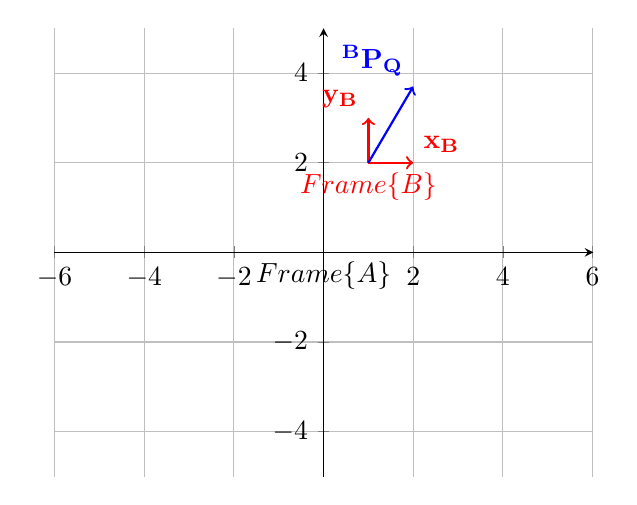
\begin{tikzpicture}
\begin{axis}[axis lines=middle, xmin=-5, xmax=5, ymin=-5,ymax=5,axis equal,grid=both]
\addplot [->, thick,  red] coordinates { (1,2) (2,2)}node[above right]{$\mathbf{x_B}$};
\addplot [->, thick,  red] coordinates { (1,2) (1,3)}node[above left]{$\mathbf{y_B}$};
\addplot [->, thick,  blue] coordinates { (1,2) (2,3.7)}node[above left]{$\mathbf{^BP_Q}$};
\addplot [red] coordinates { (1,2) (1,2)}node[below]{$Frame \{B\}$};
\addplot [black] coordinates { (0,0) (0,0)}node[below]{$Frame \{A\}$};
\end{axis}
\end{tikzpicture}\\\\\\
\textbf{Angular Velocity}\\
Consider two frames \{A\},\{B\}; where \{A\} is fixed  and \{B\} is moving away from \{A\}. No linear motion for \{B\}. Let Frame \{B\} have a point Q(${}^BP_Q$). We can compute the angular velocity of ${}^BP_Q$ with respect to frame \{A\} using the formula: \\
${}^AV_Q = {}^A_BR {}^BV_Q + {}^A_B\Omega \times {}^A_BR {}^BP_Q$

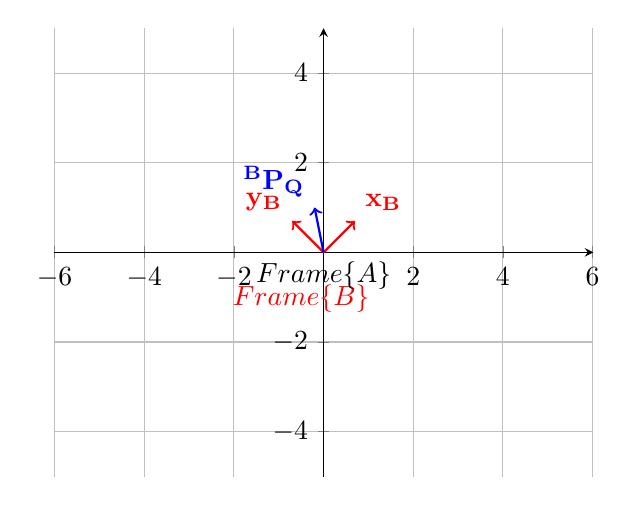
\begin{tikzpicture}
\begin{axis}[axis lines=middle, xmin=-5, xmax=5, ymin=-5,ymax=5,axis equal,grid=both]
\addplot [->, thick,  red] coordinates { (0,0) (.7,.7)}node[above right]{$\mathbf{x_B}$};
\addplot [->, thick,  red] coordinates { (0,0) (-.7,.7)}node[above left]{$\mathbf{y_B}$};
\addplot [->, thick,  blue] coordinates { (0,0) (-.2,1)}node[above left]{$\mathbf{^BP_Q}$};
\addplot [red] coordinates { (-.5,-.5) (-.5,-.5)}node[below]{$Frame \{B\}$};
\addplot [black] coordinates { (0,0) (0,0)}node[below]{$Frame \{A\}$};
\end{axis}
\end{tikzpicture}

\subsection{Velocity Propagation equations(iterative)}
1. ${}^{i+1}\omega_{i+1}={}^{i+1}_iR({}^i \omega_i) + \dot{\theta}_{i+1} {}^{i+1}\hat{z}_{i+1}$\\
2. ${}^{i+1}v_{i+1}={}^{i+1}_iR({}^i v_i + {}^i \omega_i \times {}^i P_{i+1}) + \dot{d}_{i+1} {}^{i+1}\hat{z}_{i+1}$\\\\
\begin{itemize}
    \item i is joint/frame
    \item i+1 next frame
    \item $\omega$ angular velocity
    \item $v$ linear velocity
    \item $\dot{\theta}_{i+1} \hat{z}$ is for revolute joints: $\begin{bmatrix}
        0\\
        0\\
        \dot{\theta}_{i+1}
    \end{bmatrix}$
    \item $\dot{d}_{i+1} \hat{z}$ is for prismatic joints: $\begin{bmatrix}
        0\\
        0\\
        \dot{d}_{i+1}
    \end{bmatrix}$
    \item The main idea is starting from frame \{0\} iteratively solve the sdolution for $n$ joints. 
\end{itemize}

\subsection{Example}
\includegraphics[width=10cm]{vel_prop_example.png}\\\\
\textbf{Part a}:\\
Base frame usually never moves so we can say:\textbf{frame\{0\}}\\
${}^0\omega_0={}^0v_0=\begin{bmatrix}
0\\
0\\
0
\end{bmatrix}$\\\\
\textbf{Frame \{1\}} iteration(i=0):\\
1. ${}^1 \omega_1 = {}^1_0R ({}^0 \omega_0) + \dot{\theta}_1 \hat{z} = \begin{bmatrix}
    0\\
    0\\
    \dot{\theta}_1
\end{bmatrix}$\\
2. ${}^{1}v_{1}={}^{1}_0R({}^0 v_0 + {}^0 \omega_0 \times {}^0 P_{1}) + \dot{d}_{1} {}^{1}\hat{z}_{1}=\begin{bmatrix}
    0\\
    0\\
    0
\end{bmatrix}$ $\dot{d}_{1} {}^{1}\hat{z}_{1}$ goes to zero cause revolute joint here.\\\\
\textbf{Frame \{2\}} iteration(i=1):\\
1. ${}^2 \omega_2 = {}^2_1R ({}^1 \omega_1) + \dot{\theta}_2 \hat{z} =\begin{bmatrix}
-s_2 & 0 & c_2\\
-c_2 & 0 & -s_2\\
0 & -1 & 0
\end{bmatrix} \begin{bmatrix}
    0\\
    0\\
    \dot{\theta}_1
\end{bmatrix} + \begin{bmatrix}
0\\
0\\
\dot{\theta}_2
\end{bmatrix} = \begin{bmatrix}
    c_2\dot{\theta}_1\\
    -s_2\dot{\theta}_1\\
    \dot{\theta}_2
\end{bmatrix}$\\
2. ${}^{2}v_{2}={}^{2}_1R({}^1 v_1 + {}^1 \omega_1 \times {}^1 P_{2}) + \dot{d}_{2} {}^{2}\hat{z}_{2}=
\begin{bmatrix}
-s_2 & 0 & c_2\\
-c_2 & 0 & -s_2\\
0 & -1 & 0
\end{bmatrix} (\begin{bmatrix}
    0\\
    0\\
    0
\end{bmatrix} + \begin{bmatrix}
    0\\
    0\\
    \dot{\theta}_1
\end{bmatrix} \times \begin{bmatrix}
    0\\
    0\\
    0
\end{bmatrix})=
\begin{bmatrix}
    0\\
    0\\
    0
\end{bmatrix}$ $\dot{d}_{2} {}^{2}\hat{z}_{2}$ goes to zero cause revolute joint here.\\\\

\textbf{Frame \{3\}} iteration(i=2):\\
1. ${}^3 \omega_3 = {}^3_2R ({}^2 \omega_2) + \dot{\theta}_3 \hat{z} =\begin{bmatrix}
1 & 0 & 0\\
0 & 0 & 1\\
0 & -1 & 0
\end{bmatrix} \begin{bmatrix}
    c_2\dot{\theta}_1\\
    -s_2\dot{\theta}_1\\
    \dot{\theta}_2
\end{bmatrix}  = \begin{bmatrix}
    c_2\dot{\theta}_1\\
    \dot{\theta}_2\\
    s_2\dot{\theta}_1
\end{bmatrix}$ $\dot{\theta}_{2} {}^{2}\hat{z}_{2}$ goes to zero cause prismatic joint here.\\
2. ${}^{3}v_{3}={}^{3}_2R({}^2 v_2 + {}^2 \omega_2 \times {}^2 P_{3}) + \dot{d}_{3} {}^{3}\hat{z}_{3}=
\begin{bmatrix}
1 & 0 & 0\\
0 & 0 & 1\\
0 & -1 & 0
\end{bmatrix} (\begin{bmatrix}
    0\\
    0\\
    0
\end{bmatrix} + \begin{bmatrix}
    c_2\dot{\theta}_1\\
    -s_2\dot{\theta}_1\\
    \dot{\theta}_2
\end{bmatrix} \times \begin{bmatrix}
    0\\
    \dot{d}_3\\
    0
\end{bmatrix}) + \begin{bmatrix}
    0\\
    0\\
    \dot{d}_3
\end{bmatrix}=
\begin{bmatrix}
    d_3\dot{\theta}_2\\
    -d_3c_2\dot{\theta}_1\\
    \dot{d}_3
\end{bmatrix}$ \\\\
\textbf{Part b:}\\
Find ${}^3J$. Note when solving for jacobian, you only need to use linear velocity. \\
${}^3v=\begin{bmatrix}
    d_3\dot{\theta}_2\\
    -d_3c_2\dot{\theta}_1\\
    \dot{d}_3
\end{bmatrix}=\begin{bmatrix}
0 & d_3 & 0\\
-d_3C_2 & 0 & 0\\
0 & 0 & 1
\end{bmatrix}\begin{bmatrix}
\dot{\theta}_1\\
\dot{\theta}_2\\
\dot{d}_3
\end{bmatrix} \rightarrow \dot{Y}=J\dot{X}$\\\\

\textbf{Part c:}\\
Find ${}0^J$. \\
${}^0J={}^0_3R {}^3J=\begin{bmatrix}
-c_{12} & s_1 & c_1c_2\\
-s_1s_2 & c_1 & s_1c_2\\
c_2 & 0 & s_2
\end{bmatrix}
\begin{bmatrix}
0 & d_3 & 0\\
-d_3C_2 & 0 & 0\\
0 & 0 & 1
\end{bmatrix}=\begin{bmatrix}
-s_1d_3c_2 & -c_1s_2d_3 & c_1c_2\\
-c_1d_3c_2 & -s_1s_2d_3 & s_1c_2\\
0 & c_2d_3 & s_2
\end{bmatrix}$\\\\
\textbf{Part D}\\
Find singularities by taking determinant: You must solve the unknowns in $det[{}^0J]$. You can use levitas determinant or some software. The unknowns will be $\theta_1, \theta_2, d_3$ and these are values for parameters that reduce DOF of robot(aka robot must avoid these values).


\section{Jacobian Matrix - Torques and Forces on Joints}
Two type of joints -revolute and prismatic.\\
Revolute produces torque and prismatic produces force.\\\\
\textbf{Equation:} $\tau = {}^0J \hat{F}$ where,:\\
$\tau:$ is the vector of torques and forces for each joint\\
$\hat{F}: $ the unit forces\\\\
\includegraphics[width=10cm]{torques_forces_example.png}


\section{Lagrangian Mechanics (Torques and Forces)}
\textbf{Goal:} Find the torques or forces acting on a joint\\
$\mathcal{L}=$ kinetic(KE) $-$ potential(PE)\\
\begin{itemize}
    \item KE = $\frac{1}{2}mv^2$
    \item PE = $mgh$
    \item $\theta = position$
    \item $\dot{\theta} = velocity$
    \item R $\rightarrow$ torque (revolute)
    \item P $\rightarrow$ force (prismatic)
\end{itemize}

\subsection{Algorithm}
\begin{itemize}
    \item Robot manipulator $\rightarrow$ Position vector $(\theta)$
    \item Differentiate $\rightarrow$ velocity vector $(\dot{\theta})$
    \item KE = $\frac{1}{2}mv$, PE = $mgh$
    \item $\mathcal{L}$= KE - PE
    \item $\tau = \frac{d}{dt}(\frac{\partial \mathcal{L}}{\partial \dot{\theta}}) - \frac{\partial \mathcal{L}}{\partial \theta} - $[external forces/torques]$\theta$ \textbf{or F}
\end{itemize}

\subsection{Example}
\includegraphics[width=10cm]{part1_lagrange.png}\\
\includegraphics[width=10cm]{part2_lagrange.png}\\
\includegraphics[width=10cm]{part3_lagrange.png}\\
\includegraphics[width=10cm]{part4_lagrange.png}

\section{Trajectory Planning and Generation}
\textbf{Trajectory:} Time history of position, velocity and acceleration for each DOF.\\
\begin{itemize}
    \item Run time
    \item Path update rate (60-2000hz)
    \item You also want smooth motion(minimze wear and tear)
    \item \textbf{Via points:} auxilary/intermediate points between initial and final positions
    \item Optimization problem because there are many ways to potentially go from initial to final
\end{itemize}

\textbf{Path Generation Methods}
\begin{itemize}
    \item Joint Space Schemes $\rightarrow$ using function of joint angles(in terms of $\theta$),  each via point(including final and initial) is converted to a set of joint angles using inverse kinematics
    \item Cartesian Schemes $\rightarrow$ directly uses the position and orientation of the robot frames along with the path points as specified by the user to generate the trajectory.
\end{itemize}
In general, joint space schemes are easier to use and compute. This is because cartesian schemes require inverse kinematics to be used at every single point along the path, in the path update. So higher computational burden on the robot. 

\subsection{Joint Space Schemes}
Is split into two sub methods:
\begin{itemize}
    \item Cubic Polynomials(can be even higher order)
    \item Parabolic Blends
\end{itemize}

\subsection{Cubic Polynomials}
The idea here is to find an equation(3rd degree polynomial) that satisfies the following constraints:\\
\begin{itemize}
    \item $\theta(t_0)=\theta_0$ aka the initial position at time 0 is the initial position of the robot
    \item $\dot{\theta(0)}=0$ aka the derivative of the initial postion has velocity 0
    \item $\theta(t_f) = \theta_f$ the final position at time f, is at the intended final position
\end{itemize}
To model a polynomial with 4 constraints you need at least a 3rd degree polynomial. If you add via points, then you can increase the degree of the polynomial by adding additional constraints. \\\\
\textbf{Form of functions:}\\
\begin{itemize}
    \item $\theta(t)=a_0+a_1t+a_2t^2+a_3t^3$ Position
    \item $\dot{\theta(t)}=a_1+2a_2t+3a_3t^2$ Velocity
    \item $\ddot{\theta(t)}=2a_2+6a_3t$ Acceleration
\end{itemize}
\textbf{Example:}\\
\includegraphics[width=10cm]{cubic_polynomial_example.png}

\subsection{Parabolic Blends}
To solve discontinuous velocities, we use parabolic blends.\\
\textbf{Explanation:}\\
\includegraphics[width=10cm]{parabolic_explanation.png}\\
\textbf{Example:}\\
\includegraphics[width=10cm]{parabolic_example.png}

%\section{LIE Algebra}

\section{Credit}
These are my notes from the robotics playlist youtube channel @thatsengineering5235, all of the external images used are examples from their videos. 
\end{document}
